\documentclass[assd_tp3_main.tex]{subfiles}

\begin{document}

\section{Conversores $\Sigma\Delta$}
Los conversores $\Sigma\Delta$ destacan por brindar la posibilidad de tener un buen rango dinámico siempre que
la señal a digitalizar no se extienda en un amplio rango de frecuencia.
\subsection{Error de cuantización}
La cuantización es convertir una muestra de valor continuo x a un conjunto finito de valores discretos $q_i$.
M es la cantidad de valores $q_i$ que esta determinada por el tipo de cuantizador  su funcion transferencia q(x).
Para un cuantizador uniforme, los subintervalos $\Delta=q_{i+1}-q_i$ son iguales. Este tipo de cuantizador es más común pero no siempre es el más eficiente.
La diferencia $e(n)=q_i(n)-x(n)$ se llama error de cuantización. El mismo está en el orden de $\Delta$.
Cabe aclarar que si se va de escala la señal introducida $\Delta$ toma un valor mayor que el establecido.
Como la señal digital final es representada en un valor binario de B bits entonces hay un total de $M=2^{B}$ niveles de cuantización disponibles.
Asumiendo que la secuencia x(n) es escalada de forma tal que $|x(n)|\leq1$ entonces como $x_{max} =1$ y $x_{min} =-1$:
\[ \Delta=\frac{x_{max}-x_{min}}{2^B-1} = \frac{2}{2^B-1} \]
El error de cuantización e(n) debido a que se obtiene por aproximar al valor mas cercano, tiene un máximo valor absoluto de $0.5\Delta$.
Se sigue que:
\[ x_q(n)= x(n)+e(n)\]
En donde e(n) se lo llamará de ahora en más ruido de cuantización.
\begin{figure}[H]
\centering
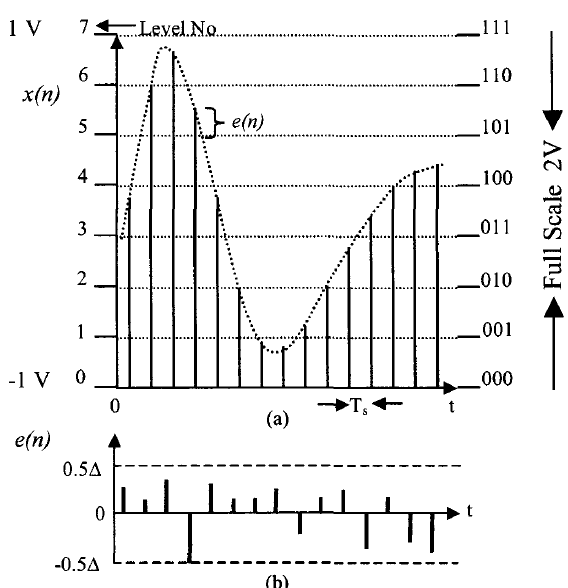
\includegraphics[width=0.52\linewidth]{images/ej4/quant_err.png}
\caption{En los procesos de cuantizacion los valores de las muestras son redondeadas al nivel más cerca disponible y luego son representadas en binario. La alteración de las muestras iniciales converge en el ruido de cuantización e(n)}
\label{fig:quant_err}
\end{figure}
El ruido de cuantización e(n) está casi incorrelacionado con la señal de entrada, tiene un espectro blanco y su distribución de probabilidad es uniforme en el rango $[-\Delta/2,\Delta/2]$.
Como consecuencia el error de cuantización puede pensarse como una fuente de ruido blanco aditivo e independiente.

Se define el SQRN como la relación Señal-Ruido de cuantización:
\[ SQNR= \frac{PotSe\tilde{n}al}{PotRuidoCuantizado}\]

\begin{figure}[H]
\centering
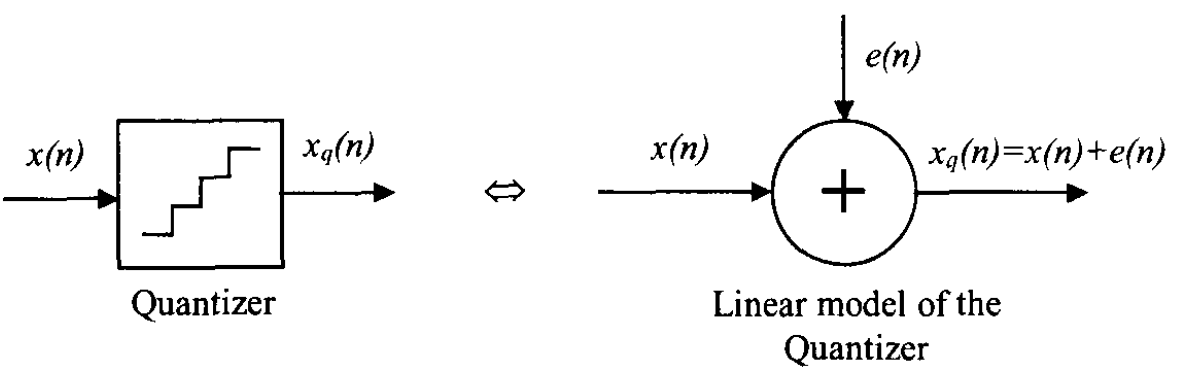
\includegraphics[width=0.52\linewidth]{images/ej4/cuantmodel.png}
\caption{Modelo lineal para el cuantizador}
\label{fig:cuantmodel}
\end{figure}


Por ser uniforme en $[-\Delta/2,\Delta/2]$:\\
\[ \mu_e = 0 \]
\[ \sigma_e^2 = \frac{\Delta^2}{12} \]
Si los valores de e(n) se asumen incorrelacionados e identicamente distribuidos el ruido de cuantización es blanco y su potencia es distribuida uniformemente sobre todo el rango de $[-f_s/2,f_s/2]$. Por tanto, la densidad espectral de potencia en el ruido N(f) puede ser expresada como:
\[ N(f)=\frac{\Delta^2}{12f_s} \]
Para una senoidad con variación de amplitud en escala completa\\ 
$2A =(2^B-1)\Delta$, su potencia es $A^2/2$ y el SQRN es:\\
\[ SQRN=10log\left( \frac{A^2/2}{\sigma_e^2} \right)\approx10log\left(\frac{3\cdot2^{2B}}{2}\right)=(6.02 \cdot B+1.76)dB \]
Se concluye que si se incrementa en uno el número de bits, se aumenta el SQNR en 6dB.
De hecho, esto nos da pie a pensar el máximo número de bits que se necesita para cuantizar una señal analógica con un piso de ruido específico.
Una característica que se debe destacar de un cuantizador es su rango dinámico. 
\[ rango\,dinamico=log_2\frac{x_{max}}{\Delta/2}\]

\begin{figure}[H]
\centering
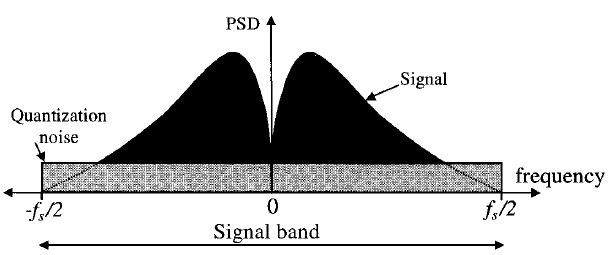
\includegraphics[width=0.52\linewidth]{images/ej4/ruido_desplazado.png}
\caption{Densidad espectral de potencia en la salida de un ADC convencional. El ruido de cuantización se distribuye en toda la banda de la señal}
\label{fig:PSD}
\end{figure}

\subsection{Principios de Oversampling}
Los requerimientos de alta resolución y rango dinámico en el procesamiento de señales no puede ser logrado con los ADCs convencionales, debido a las limitaciones de sus implementaciones.\\
Algunos problemas que suelen presentar son los siguientes:
\begin{itemize}
\item La implementación de cuantizadores uniformes con un gran número de niveles de cuantización. Para un SAR ADC con 16 bits de precisión, $2^{16}=65536$ niveles equidistantes deben ser determinados.
\item La implementación del FAA con requerimientos estrictos tales como una banda angosta de transición, alta atenuación en la banda de rechazo, muy poco ripple en la banda pasante ,fase lineal, bajo ruido, etc. Tales especificaciones no se pueden lograr con circuitos integrados analógicos.
\item La presencia del efecto Jitter, por ejemplo la incertidumble en el tiempo de flancos del pulso de clock usados en el muestreador. 
\end{itemize}
Una manera de mejorar esta situación es incrementar la tasa de muestreo mucho más que la de los ADCs convencionales, por ejemplo arriba de Nyquist $(f_{N}=2f_b)$. Muestrear a una $f_s$ mas grande que la de Nyquist se la suele llamar $\bold{oversampling}$.
Una medida del oversampling es la llamada Oversampling Ratio (OSR) definida como R:
\[ R=\frac{f_s}{f_N} \]
En general R es un número potencia de 2. Si el R está entre 2 y 16 hablamos de un grado leve de oversampling mientras que un grado elevado de oversampling ocurre cuando R está entre 16 y 256.

\begin{figure}[H]
\centering
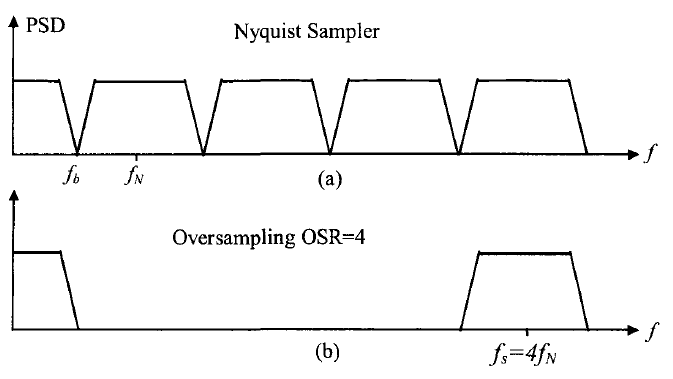
\includegraphics[width=0.52\linewidth]{images/ej4/oversampling.png}
\caption{El proceso de oversampling separa las bandas de la señal}
\label{fig:oversampling}
\end{figure}

En la figura \ref{fig:oversampling} se puede ver que las bandas no están muy cercanas a otras, lo cual nos permite tener una frecuencia en el FAA mayor.
Además cuando el oversampling es utilizado, la potencia del ruido de cuantización se distribuye en un rango más amplio de frecuencia lo que provoca que su efecto se vea en menor proporción.
El ruido de cuantización que queda afuera de la banda de la señal puede ser eliminada con un filtro digital de alta precisión. 

\[ SQNR_{Oversampling}=10log\frac{A^2/2}{(\Delta^2/12)/R}=SQNR_{Nyquist}10log(R) \]

Entonces se conluye que frente a una igual cantidad de bits se tiene mejor precisión utilizado el concepto de oversampling.

\begin{figure}[H]
\centering
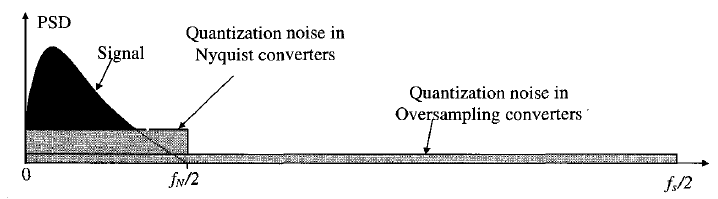
\includegraphics[width=0.8\linewidth]{images/ej4/oversampling_noise.png}
\caption{Cuando se incrementa en 4 la tasa de muestreo, el ruido de cuantización se distribuye sobre una región más grande. En consecuencia, la potencia del ruido de cuantizacion es 4 veces menor}
\label{fig:oversampling_noise}
\end{figure}

\todo[inline]{aca se supone que vendria el modulador delta}

\subsection{Concepto de Noise Shaping}
Una última mejora en el SQNR puede ser lograda mediante el desplazamiento del ruido que se encuentra en la banda de la señal. Esto se puede lograr fácilmente si STF(z) es un pasa todo mientras que NTF(z) es un pasa altos.
Esta técnica se conoce como Noise Shaping y puede ser facil y eficientemente implementada por una modificación en el sistema DM. Si en el diagrama en bloques del modulador delta colocamos otro integrador después de la x(n), lo que se obtiene finalmente es STF(z) y NTF(z) de la forma que queríamos.
\begin{figure}[H]
\centering
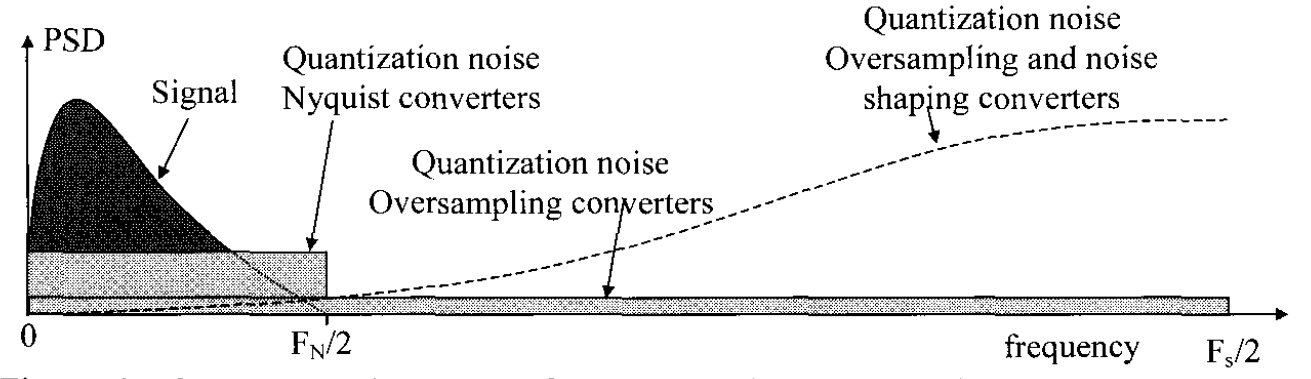
\includegraphics[width=0.8\linewidth]{images/ej4/noise_shaping.png}
\caption{Espectro de la salida de un cuantizador con noise shaping comparado con el de los conversores Nyquist y con Oversampling implementado }
\label{fig:noise_shaping}
\end{figure}

\begin{figure}[H]
\centering
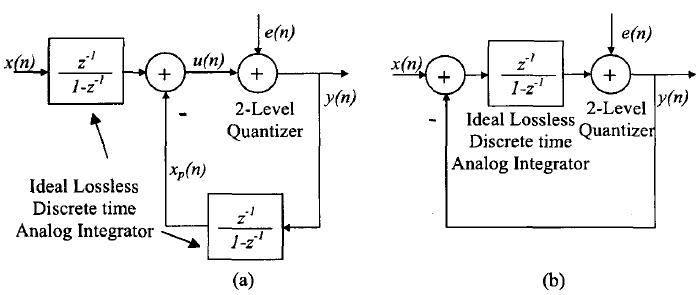
\includegraphics[width=0.6\linewidth]{images/ej4/sd_block_model.png}
\caption{Desarrollo sucesivo del esquema $\Sigma\Delta$ }
\label{fig:sd_block_model}
\end{figure}

\subsection{Decimación: Introducción teórica}
El general se suele hacer un oversampling de una señal y luego reducir la frecuencia de muestreo hasta la de Nyquist en el caso de un ADC o incrementarlo en caso de un DAC se llama. La primera opción es llamada decimación mientras que a la otra se la llama interpolación.
Esas tasas de muestreo pueden ser implementadas utilizado filtros FIR de alta precisión, usualmente en distintas etapas.
Usualmente la decimación es aplicada en la salida del sigma delta para facilitar la conversión A/D y dar una señal multibit que se encuentra en la banda la frecuencia de muestreo de Nyquist.
\subsubsection{Rate Conversion}
Hay varios casos donde la tasa de muestreo ne la cual las señales digitales son procesadas necesitan ser cambiadas. Surgen esas necesidades cuando se interfacean dos sistemas con dos tasas de muestreo distintos. El proceso en el cual  la tasa de muestreo es reducido r veces se llama decimación, \textbf{debido a que se guarda solo una de cada r muestras}.
El proceso inverso de aumentar la tasa de muestreo por r, se llama interpolación, debido a que se insertan r-1 muestras apropiadas entre dos muestras originales.
\subsubsection{Decimación}
Una de cada r muestras se guardan, el resto se descartan. 
De esta forma, $f_s<=f_s/r$. Para evitar aliasing hay que colocar un filtro antialiasing en fs/2r.
\todo[inline]{foto de antialiasing}

\subsubsection{Filtros de decimación}
Un filtro pasa bajos es utilizado en el proceso de decimación. La reducción en r, divide la zona original de nyquist (0,$f_s/2$) en r zonas $(mf_s/2r,(m+1)f_s/2r)$, m=0,...,r-1. Las r-1 zonas (m=0,...,r-1) provocan aliasing a la primera, por lo tanto el contenido en esas sonas tiene que ser suprimido debajo de un nivel determinado para que la señal se pueda considerar libre de ruido. Como el ancho de banda de la señal usualmente no cubre todo el espectro de la zona de Nyquist las zonas que deben ser suprimidas son:

\[ (m\frac{f_s}{r}-\frac{B}{2},m\frac{f_s}{r}+\frac{B}{2}) \]
donde:\\
m = 1,...,
r/2 si r es par
(r-1) si r es impar 
La frecuencia de corte debe ser de B/2 y debería llegar a máxima atenuación en $f_s/r-B/2$.
\subsubsection{Filtros Comb}
En casos donde la relación R suele ser grande, la conversión suele hacerse en multiples etapas, con la etapa de más relación implementada por un filtro comb.
Los filtros comb son filtros low-pass FIR cuya funcion transferencia es:
\[ H(z)=(\frac{1}{r}suma z^{-i})^N=(\frac{1}{r}\frac{1-z^-{r}}{1-z^{-1}})^N \]
Como todos los coeficientes son unitarios, se pueden implementar facilmente.
El denominador está implementado como integrador en la relación mas grande, mientras el numerador es implementado ocmo diferenciador a la relación más chica. El orden del filtro comb es elegido igual al la tasa de conversion r, de forma tal que los zeros de la ecuación sean multiplos de $f_s/r$.
\subsection{Simulaciones}
\subsubsection{Respuesta al impulso}
\begin{figure}[H]
\centering
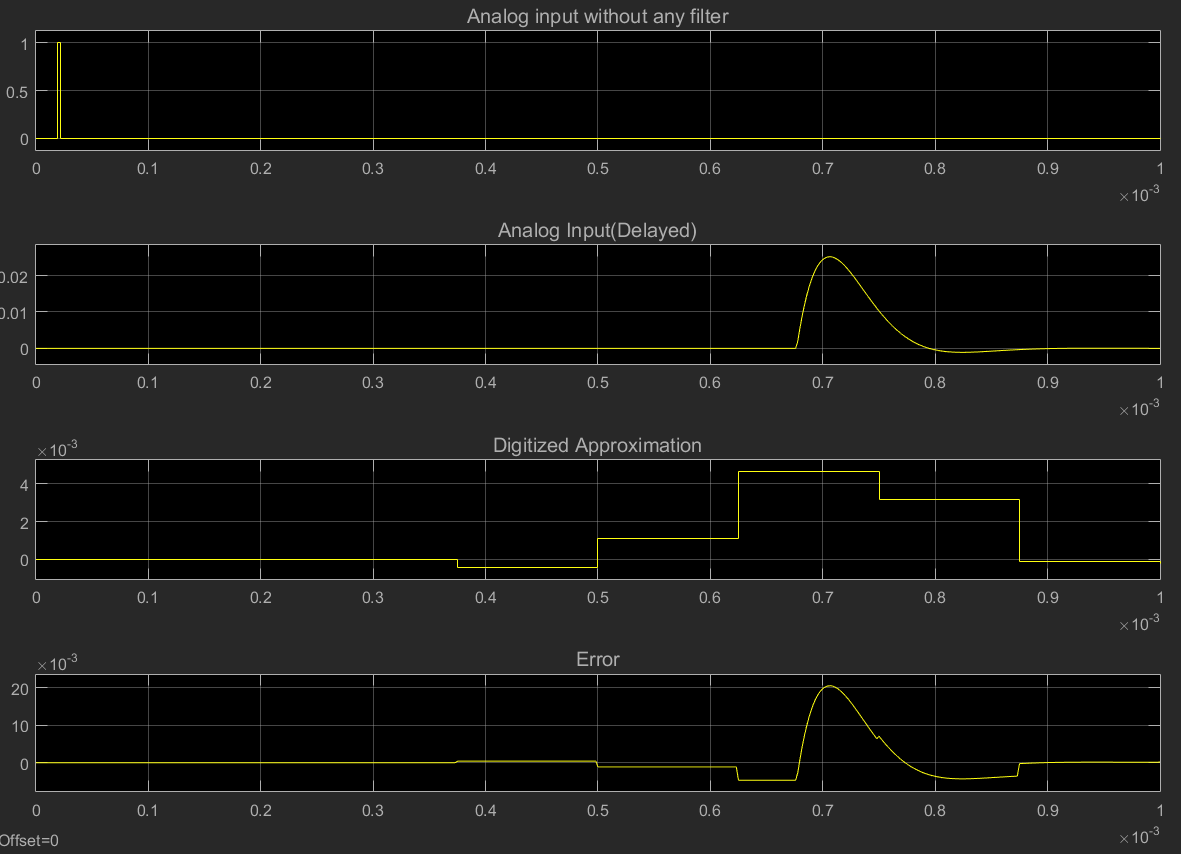
\includegraphics[width=1\linewidth]{images/ej4/impulse_response.png}
\caption{Respuesta al impulso del sistema}
\label{fig:impulse_response}
\end{figure}

\begin{figure}[H]
\centering
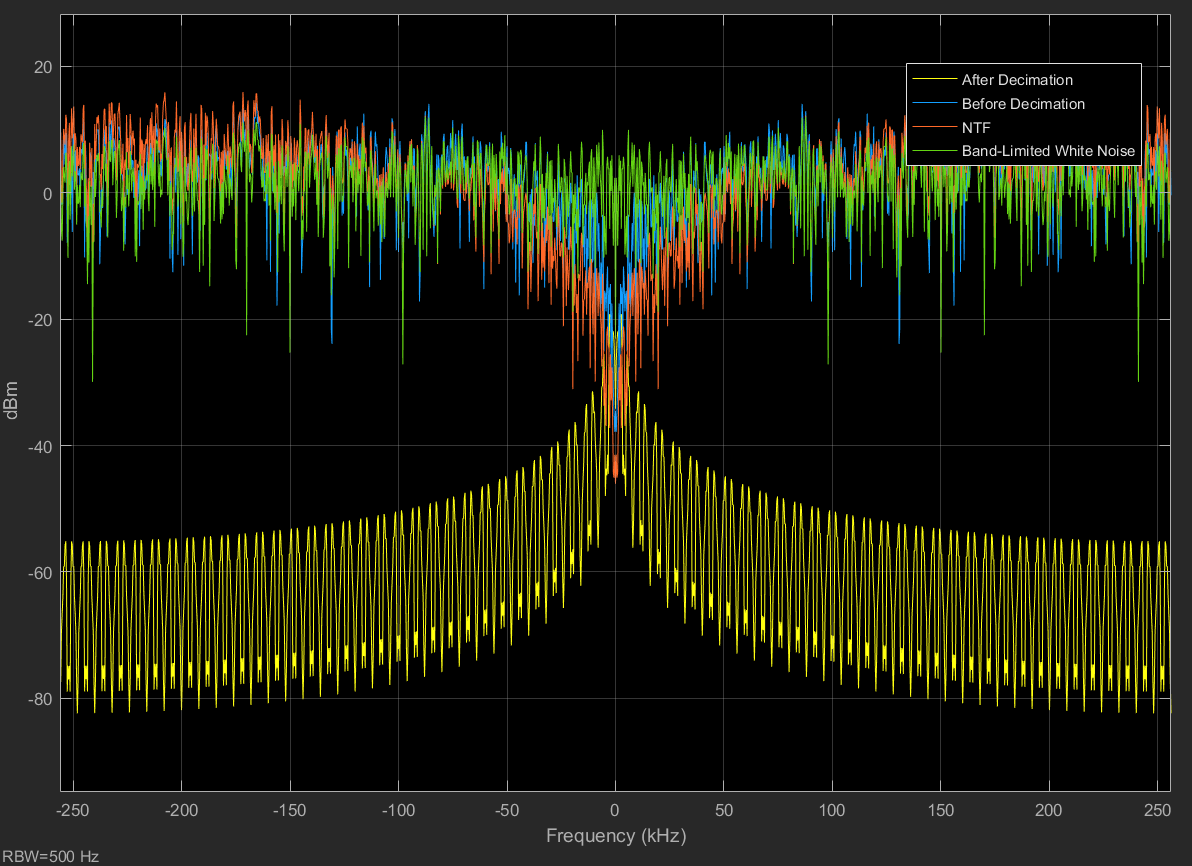
\includegraphics[width=1\linewidth]{images/ej4/NTF.png}
\caption{Espectro del Ruido de cuantización, antes de la decimación, después de la decimación y la respuesta de NTF frente al ruido}
\label{fig:NTF}
\end{figure}

\begin{figure}[H]
\centering
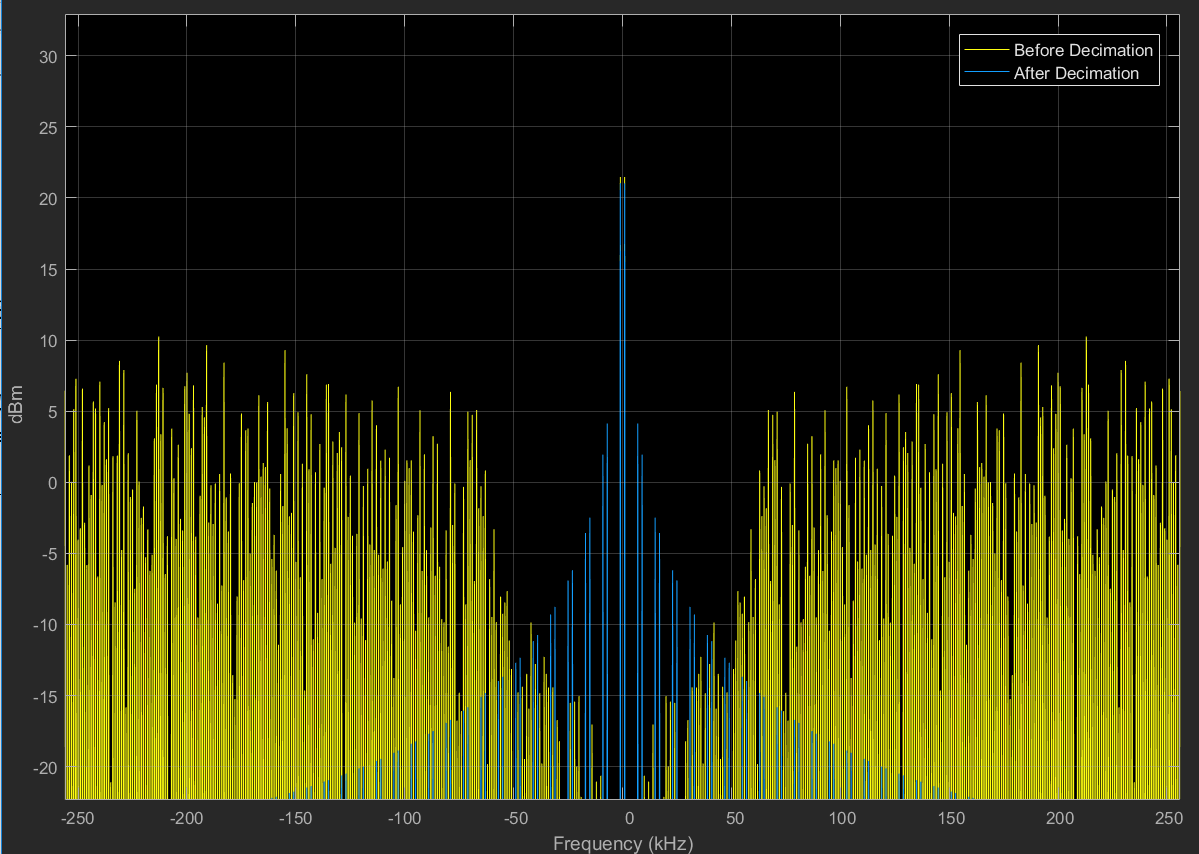
\includegraphics[width=1\linewidth]{images/ej4/sin_response_1K.png}
\caption{Respuesta a una senoidal de 1KHz}
\label{fig:sin_response_1K}
\end{figure}

\begin{figure}[H]
\centering
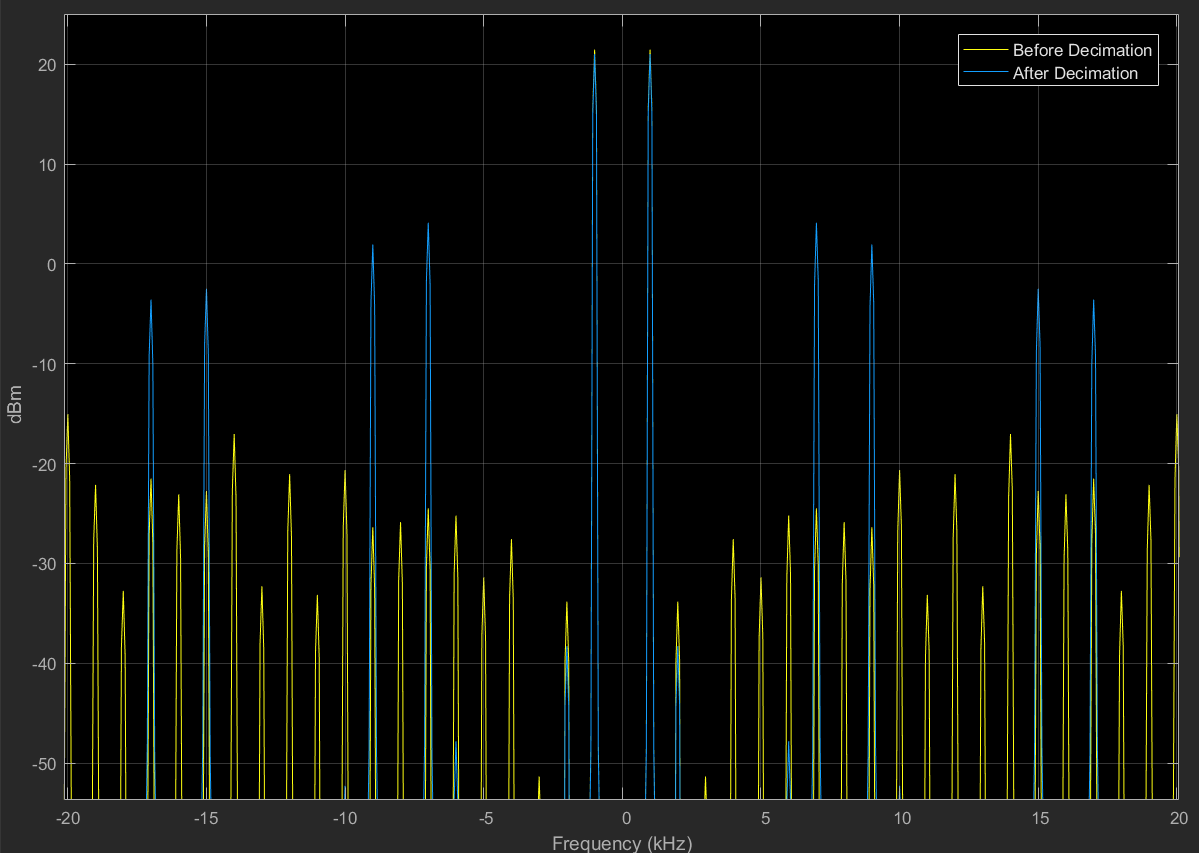
\includegraphics[width=1\linewidth]{images/ej4/sin_response_1K_zoom.png}
\caption{Respuesta a una senoidal de 1KHz (con zoom)}
\label{fig:sin_response_1K_zoom}
\end{figure}





\subsection{Moduladores $\Sigma\Delta$ de primer orden }
Recordamos dos características importantes del modulador:
\begin{itemize}
\item \textbf{Oversampling}: distribuye el ruido de cuantización 
\item \textbf{Noise shaping}: expulsa la mayoría del ruido que estaba dentro de la banda a frecuencias altas. 
\end{itemize}
A continuación se presentan diagramas en bloques del modulador $\Sigma\Delta$ de primer orden.
\begin{figure}[H]
\centering
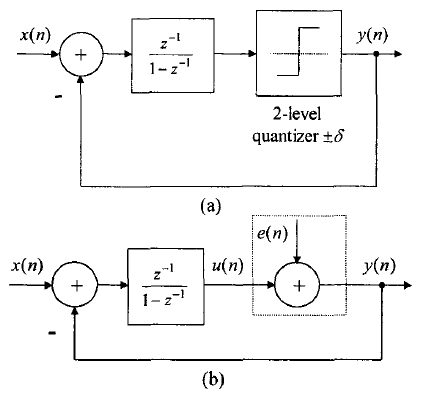
\includegraphics[width=0.4\linewidth]{images/ej4/sd_linmodel.png}
\caption{Diagrama en bloques del modulador $\Sigma\Delta$(a) y su modelo lineal(b)}
\label{fig:sigmadelmod_model}
\end{figure}
La señal e(n) en el modelo lineal de la figura \ref{fig:sigmadelmod_model} se la llama ruido de cuantización.
\[ y(n)=x_q(n)= u(n)+e(n) \]
De la figura \ref{fig:sigmadelmod_model} obtenemos la SignalTransferFunction (STF) y la NoiseTransferFunction (NTF):
\[ Y(z)= z^{-1}X(z)+(1-z^{-1})E(z) \]
\[ STF(z)= z^{-1} \]
\[ NTF(z)= 1-z^{-1} \]


\end{document}
